%%==================================================================%%
%% Author : Tejedo Gonz�lez, Daniel                                 %%
%%          S�nchez Barreiro, Pablo                                 %%
%% Version: 1.0, 25/11/2012                                         %%
%% Version: 2.0, 06/02/2013                                         %%
%%                                                                  %%
%% Memoria del Proyecto Fin de Carrera                              %%
%% Sintaxis abstracta, archivo ra�z                                 %%
%%==================================================================%%

\chapterheader{Desarrollo de la Sintaxis Abstracta}{Desarrollo de la Sintaxis Abstracta}
\label{chap:metamodelo}

El presente cap�tulo describe el proceso de desarrollo de nuestra primera tarea de acuerdo al proceso de desarrollo dirigido por modelos de nuestro lenguaje. Dicha tarea es el desarrollo de un metamodelo o sintaxis abstracta para nuestro lenguaje.

\chaptertoc

\section{Introducci�n}
\label{sec:meta:requisitos}
\todo{Escribir una introducci�n, que es como un mini toc pero con m�s detalle describiendo la estructura de cap�tulo. Al final de la secci�n, describe la estructura del cap�tulo}
%%%==================================================================%%
%% Author : Tejedo González, Daniel                                 %%
%%          Sánchez Barreiro, Pablo                                 %%
%% Version: 1.0, 27/11/2012                                         %%
%% Version: 2.0, 09/03/2013                                         %%
%%                                                                  %%
%% Memoria del Proyecto Fin de Carrera                              %%
%% Gramática, Introduccion                                          %%
%%==================================================================%%


De acuerdo con la metodolog��a impuesta por la Ingenier�a de Lenguajes Dirigida por Modelos, el siguiente paso para desarrollar el lenguaje HCL pasa por desarrollar una sintaxis textual que sea capaz de vincular el metamodelo construido con las l�neas de c�digo que escribamos en nuestro lenguaje.  Esta sintaxis textual se construye a trav�s de una gram�tica, en la que especificamos una serie de reglas para cada una de las metaclases, de modo que esas reglas satisfagan la sintaxis y los requisitos de nuestro lenguaje. 

%%==================================================================%%
%% NOTA(Pablo): Cuando llegues a la parte en la cual hablas de      %%
%%              requisitos insertas esto                            %%
%%==================================================================%%

Los requisitos que nuestra gram�tica debe cumplir ya estaban pr�cticamente definidos, pues la gram�tica BNF definida por el profesor Pablo S�nchez, mostrada en la Figura~\ref{fig:constraintBNF}, es m�s o menos la misma que hemos tenido que implementar (con la salvedad que a�ade cambiar de lenguaje BNF a EMFText).

No obstante, hubo que a�adir una serie de consideraciones adicionales para refinar dicha gram�tica. Concretamente, tuvimos que a�adir los siguientes requisitos a la notaci�n BNF de nuestra gram�tica:

\begin{itemize}
    \item Deb�a permitirse la posibilidad de especificar prioridad en las operaciones, es decir, de poder delimitar las operaciones con par�ntesis que denoten el orden de realizaci�n de las mismas.
    \item Todo fichero de especificaci�n de restricciones debe comenzar con una l�nea que indique la ruta donde se encuentra el �rbol de caracter�sticas al que han de aplicarse las restricciones. La sintaxis de este aspecto ser� $import ruta$, donde ruta es una direcci�n que indique un fichero en nuestro computador.
    \item Todas las restricciones han de separarse entre ellas mediante el car�cter `\texttt{;}'.
\end{itemize}

%%==================================================================%%
%% NOTA(Pablo): y luego sigue con la introducción                   %%
%%==================================================================%%

Para hablar de la gram�tica, el cap�tulo se estructurar� del siguiente modo: Tras esta introducci�n, habr� una secci�n en la que se hablar� de la implementaci�n de la gram�tica. Se explicar� paso a paso cada una de las l�neas que la componen, adem�s de su relaci�n con el metamodelo. A continuaci�n, se hablar� en otra secci�n de las pruebas a las que fue sometida la gram�tica para corroborar su correcto funcionamiento.

\section{Captura de requisitos}
\label{sec:meta:requisitos}
%%==================================================================%%
%% Author : Tejedo Gonz�lez, Daniel                                 %%
%%          S�nchez Barreiro, Pablo                                 %%
%% Version: 1.0, 25/11/2012                                         %%
%% Version: 2.0, 06/02/2013                                         %%
%%                                                                  %%
%% Memoria del Proyecto Fin de Carrera                              %%
%% Sintaxis abstracta, requisitos                                   %%
%%==================================================================%%

El primer paso para desarrollar nuestro lenguaje era conocer qu� aspecto deb�a tener nuestro lenguaje y qu� restricciones deb�a satisfacer. Es decir, en primer lugar debemos realizar un proceso que podemos denominar de captura de requisitos para poder comprender qu� es lo que tiene que hacer exactamente el lenguaje que se pretende crear.

Concretamente nuestro lenguaje hab�a sido pr�cticamente definido por el profesor Pablo S�nchez, del Departamento de Matem�ticas, Estad�stica y Computaci�n de la Universidad de Cantabria, mediante notaci�n BNF. Las ideas subyacentes a dicho lenguaje son las que se describen a continuaci�n.

%%==================================================================%%
%% NOTA(Pablo): Aqu� traduce la secci�n III del art�culo que te
%%              env�o adjunto. Si te hacen falta las fuentes del
%%              art�culo, me las pides.
%%
%%              Traduce primero del ingl�s y luego lo repasas y lo
%%              reescribes para que suene a castellano
%% 
%%              Si en la secci�n III no aparecen las razones por 
%%              las cuales una caracter�stica es clonable, buscar 
%%              en qu� parte del art�culo aparecen y explicarlo

%%==================================================================%%

Adem�s nuestro lenguaje deb�a permitir vincular un un modelo de caracter�sticas sobre el cual se definir�n un conjunto de restricciones externas. Este modelo se utilizar�, por ejemplo, para comprobar que los s�mbolos que aparecen como nombres de caracter�sticas en las restricciones se refieren a caracter�sticas que realmente existen en el �rbol de caracter�sticas. Por ejemplo, una restricci�n del tipo $AdvancedHeating => Heating$ carecer�a de sentido si algunas de las caracter�sticas $AdvancedHeating$ o $Heating$ no apareciesen en el �rbol de caracter�sticas sobre el cual estamos definiendo restricciones.

%%======================================================================================%%
%% NOTA(Pablo): Esto posiblemente sobre al introducir la traducci�n de la Secci�n III.
%%              Si es as�, eliminarla.
%%              Si los conceptos de restricci�n con contexto y operaci�n cuantificada
%%              no apareciesen, meter esta clasificaci�n pero resumida
%%======================================================================================%%
%%
%% De entre todos esos requisitos b�sicos, es necesario entrar en detalle en el n�mero 3
%% y enumerar la lista de operaciones que pueden ser definidas por nuestro lenguaje. Se
%% pueden clasificar en los siguientes tipos: \\
%%
%% - L�gicas: Son operaciones cuyos operandos han de ser caracter�sticas sin
%%   cardinalidad (tambi�n llamadas caracter�sticas simples), y que se evaluan a
%%   verdadero o falso. Entre las operaciones l�gicas encontramos las cl�sicas not,
%%   and, or, xor e implica.
%%
%% - Num�ricas: Sus operandos han de ser caracter�sticas con cardinalidad (tambi�n
%%   llamadas caracter�sticas m�ltiples) o simplemente n�meros. Su resultado se evalua
%%   con un valor num�rico. Las operaciones num�ricas a implementar son la suma, resta,
%%   multiplicaci�n y divisi�n.
%%
%% - Comparativas: Sus operandos han de ser caracter�sticas m�ltiples o simplemente n�meros,
%%   pero su resultado se evalua con un valor booleano. Las operaciones de comparaci�n a
%%   implementar son igual que, mayor que, menor que, distinto que, mayor o igual que y menor
%%   o igual que.
%%
%% - Operaci�n de contexto: Operaci�n que permite hacer referencia a una caracter�stica
%%   hija de otra caracter�stica. Esta operaci�n tiene sentido para seleccionar
%%   caracter�sticas cuyo nombre pueda estar repetido pero que tengan contextos diferentes.
%%   Por ejemplo, en el modelo de caracter�sticas SmartHome de la figura \ref{figsmarthome}
%%   podemos observar que la caracter�stica HeaterMng est� presente en muchos contextos
%%   diferentes. Esta operaci�n es necesaria para poder saber con seguridad a cual de esos
%%   contextos estamos aplicando la restricci�n.
%%
%% - Operaci�n de selecci�n: Operaci�n que corresponde a los operadores l�gicos cl�sicos
%%   "para todo" o "existe", y que tiene la misma funcionalidad. Evalua si una restricci�n
%%   se cumple para todos los casos en que puede existir  o si se cumple en alguno de los
%%   casos. Por ejemplo, en el modelo de la figura \ref{figsmarthome} se podr�a evaluar una
%%   restricci�n para cada una de las habitaciones que hayan sido definidas, y saber si se
%%  cumple en todas, en alguna o en ninguna.
%%
%%======================================================================================%%

Utilizando esta informaci�n como base, procedimos a crear el correspondiente metamodelo en Ecore para nuestro lenguaje.




\section{Creaci�n del metamodelo}
\label{sec:meta:creacion}
%%==================================================================%%
%% Author : Tejedo Gonz�lez, Daniel                                 %%
%%          S�nchez Barreiro, Pablo                                 %%
%% Version: 1.0, 25/11/2012                                         %%                   %%                                                                  %%
%% Memoria del Proyecto Fin de Carrera                              %%
%% Sintaxis abstracta, creacion metamodelo                                      %%
%%==================================================================%%

Una vez hemos definido cuales son los requisitos del lenguaje, tenemos que construir nuestro metamodelo de tal modo que se ajuste a ellos y sea capaz de cumplirlos. El requisito m�s complejo y que requerir� m�s desaf�os de dise�o es, evidentemente, el de implementar todas las operaciones. As� que empezaremos primero por las partes m�s f�ciles.

Todas las restricciones que sean definidas en cada sintaxis concreta han de ser aplicadas al mismo modelo de caracter�sticas (aunque a varias configuraciones si as� lo desea el usuario). Por lo tanto, la informaci�n relativa al modelo de caracter�sticas sobre el que queremos aplicar esas restricciones es susceptible de ser almacenada en el metamodelo de nuestro lenguaje. Se entiende que el modelo de caracter�sticas que hay que guardar habr� sido previamente creado usando la herramienta Hydra, pues este editor es una extensi�n de la misma. Eso reduce mucho el n�mero de factores de los que hay preocuparse, vi�ndose reducidos en este punto a tener que almacenar �nicamente la localizaci�n del fichero dentro del sistema, para luego poder cargarlo en partes de validaci�n posteriores.

As� pues, nuestra clase inicial Model, que representa el modelo sobre el que aplicaremos las restricciones, tiene un atributo featureList en el que se guardar� la direcci�n del fichero del modelo de caracter�sticas Hydra.

Para permitir que sobre ese modelo que ya hemos representado se puedan definir un n�mero indeterminado de restricciones, es necesario crear una clase Constraint, y relacionar la clase Model con ella. La relaci�n resultante se podr�a expresar como "un modelo tiene de 0 a x restricciones", donde x es cualqueir n�mero entero positivo. 

El requisito correspondiente a la validaci�n de las restricciones que hayamos definido no tiene modo de ser resuelto a estas alturas del desarrollo de nuestra aplicaci�n, por lo que �nicamente queda la implementaci�n de las operaciones. L�gicamente, esta es la tarea de mayor complejidad de nuestro sistema. 

El primer paso es definir toda la estructura necesaria para la implementaci�n de las operaciones, haciendo que cada una de ellas est� representada en nuestro metamodelo mediante una clase, pero sin preocuparnos todav�a por las relaciones entre ellas. La clase ra�z de toda esta estructura es Operand. Es una clase abstracta, es decir, en los modelos que luego instanciemos de este metamodelo no podr� haber ninguna instancia de Operand, s�lo de los hijos no abstractos que tenga. A medida que vayamos definiendo clases hijas  de Operand estaremos especificando cada vez con m�s exactitud a qu� tipo de operaci�n estamos haciendo referencia.

En el segundo nivel de la estructura de implementaci�n de las operaciones hacemos una ramificaci�n seg�n el tipo del valor de retorno o de evaluaci�n de las posibilidades. Es decir, a la clase Operand le a�adiremos dos hijos: BoolOperand para operaciones que se eval�an a booleano y NumOperand para operaciones que se eval�an a num�rico. Estas clases tambi�n ser�n abstractas.

\begin{figure}[t]
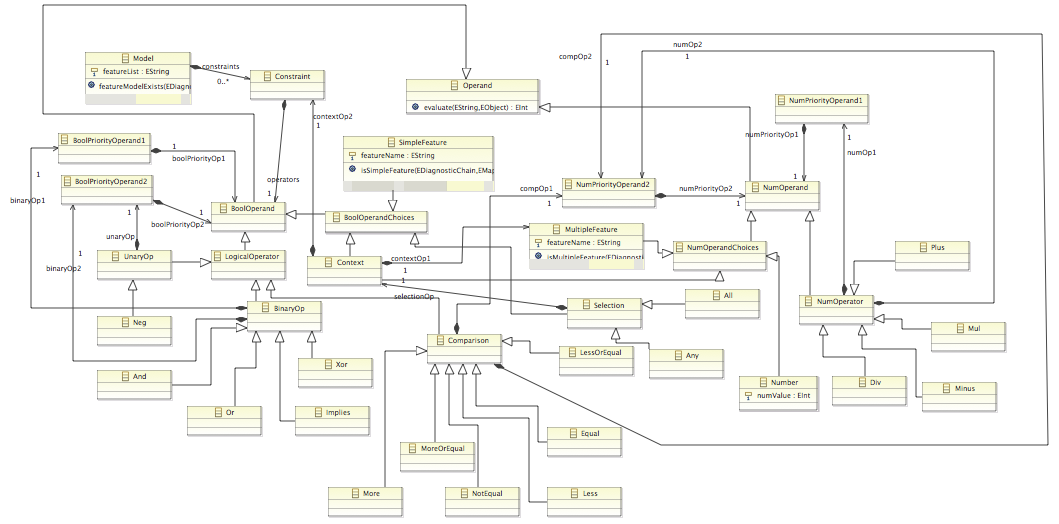
\includegraphics[scale=0.4]{metamodelo/metamodelo.jpg}
\caption{Metamodelo utilizado para la creaci�n de nuestro lenguaje de especificaci�n y validaci�n de restricciones}
\label{figmetameta}
\end{figure}


El proceso de divisi�n a partir de aqu� es m�s o menos an�logo para todas las operaciones, as� que vamos a centrarnos �nicamente en la rama que da lugar a las operaciones binarias l�gicas, para comentar despu�s los casos y situaciones especiales. Una vez tenemos la clase BoolOperand, podemos especializarla un poco m�s a LogicalOperator, que a su vez se dividir� en operaciones unarias, binarias, o de comparaci�n. Todas ellas son clases abstractas. Por fin, la clase BinaryOp heredar� las clases de las operaciones propiamente dichas, en este caso And, Or, Implies y Xor. Estas ya podr�n ser instanciadas en las sintaxis concretas que creemos.

Cabe hacer menci�n tambi�n a las clases SimpleFeature, MultipleFeature y Number, que representan a las caracter�sticas simples, m�ltiples y n�meros respectivamente. En cualquier �rbol resultante de parsear nuestro lenguaje, estas clases representar�n las hojas. En �ltima instancia todas las operaciones tendr�n como operandos caracter�sticas o n�meros. Podemos observar que SimpleFeature es un operando booleano (est� en la parte estructural de las operaciones booleanas) ya que su evaluaci�n ser� verdadero o falso, dependiendo si esa caracter�stica ha sido seleccionada en la configuraci�n correspondiente o no. MultipleFeature sin embargo se eval�a a n�mero entero. Su valor ser� el n�mero de apariciones de esa caracter�stica dentro de la configuraci�n correspondiente.

Muchas de las clases que ahora se pueden contemplar en el metamodelo de la figura \ref{figmetameta} a�n no estaban presentes en esta etapa temprana del dise�o, y su inclusi�n fue necesaria a ra�z de la creaci�n de la gram�tica y los problemas que se observaron en ese punto. En particular, las terminadas en Choices y en PriorityOperand. Las operaciones All, Any y Context en este momento eran simples herencias de BoolOperand. El motivo de estas modificaciones ser� explicado en el cap�tulo siguiente. 

Para terminar este apartado, vamos a hablar de las relaciones entre las diferentes clases de nuestro metamodelo. En este punto del dise�o no eran las mismas que las de la figura \ref{figmetameta} por los motivos explicados anteriormente. Simplemente busc�bamos una forma de relacionar cada operaci�n con los tipos de sus operandos (que tambi�n pueden ser operaciones, como es l�gico). Las operaciones l�gicas binarias tendr�n dos operandos que tambi�n ser�n binarios. En este momento del dise�o binaryOp1 y binaryOp2 iban relacionados a BoolOperand. Del mismo modo que unaryOp. Del mismo modo, compOp1, compOp2, numOp1 y numOp2 (es decir, los operandos de operaciones de comparaci�n y num�ricas respectivamente) estaban relacionados con la clase NumOperand.

La relaci�n de toda estructura de operaciones con los dos elementos anteriores, Model y Constraint, se realiza entre Constraint y BoolOperand. Toda restricci�n en �ltima ha de ser evaluada a verdadero o falso, es por eso que la relaci�n no va con Operand, como podr�a pensarse en primera instancia. De este modo estamos forzando que la operaci�n con menos profundidad del �rbol parseado de nuestra restricci�n sea booleana, y que por lo tanto el resultado final de validar la restricci�n sea un dato booleano. 

Quiz�s a alguien le pueda sorprender el hecho de que la relaci�n "operators" entre Constrain y BoolOperand sea 1..1 y no 1..*. El motivo es que como los operadores de esa primera operaci�n booleana que estamos forzando pueden ser a su vez operaciones, la complejidad en la restricci�n que podemos definir se propaga por ah� en lugar de por la relaci�n creada.







\section{Especificaci�n de Restricciones Externas}
\label{sec:emfvf:req}
%%==================================================================%%
%% Author : Tejedo Gonz�lez, Daniel                                 %%
%%          S�nchez Barreiro, Pablo                                 %%
%% Version: 1.0, 28/11/2012                                         %%
%% Version: 2.0, 06/02/2013                                         %%
%%                                                                  %%
%% Memoria del Proyecto Fin de Carrera                              %%
%% Validation Framework, implementacion                             %%
%%==================================================================%%

La sintaxis propia de Ecore no nos permite especificar ciertas restricciones que debe satisfacer nuestro metamodelo. Dichas restricciones, las cuales se enumeran a continuaci�n, deben comprobar que:

\begin{enumerate}
    \item La ruta que indica donde est� el �rbol de caracter�sticas al que se
        aplican las restricciones definidas es correctas. Ello implica comprobar tanto que la ruta es correcta como que el fichero que se halla en dicha ruta corresponde de verdad a un �rbol de caracter�sticas.
    \item El atributo \emph{featureName} asociado a una \emph{SimpleFeature} o a una \emph{MultipleFeature} corresponde al nombre de una caracter�stica perteneciente al �rbol de caracter�sticas referenciado.
    \item Una caracter�stica identificada como \emph{SimpleFeature} en el modelo de restricciones (eval�a a verdadero o falso) es realmente una caracter�stica simple (no clonable) en el �rbol de caracter�sticas asociado. Sin esta comprobaci�n, podr�amos, por ejemplo, introducir caracter�sticas m�ltiples como operandos de operadores booleanas como \emph{and} u \emph{or}. En ese caso, ser�a imposible evaluar dichas operadores ya que no podemos evaluar sus operandos a verdadero o falso.
\end{enumerate}

Respecto a la segunda restricci�n, merece la pena aclarar que el caso contrario, comprobar que una caracter�sticas considerada como m�ltiple en una restricci�n realmente lo sea, no es necesario controlarlo. La raz�n es que las caracter�sticas simples pueden tratarse como un caso particular o subtipo de caracter�stica m�ltiples, ya que siempre podremos considerarla como una caracter�stica clonable con cardinalidad $<0,1>$.

Para implementar estas restricciones externas se ha utilizado \emph{EMF Validation Framework}, herramienta integrada en EMF para este prop�sito concreto. Siguiendo las instrucciones proporcionadas por esta herramienta, a�adimos un m�todo de validaci�n a cada metaclase que necesitaba ser validada. En nuestro caso, dichas clases eran \emph{Model}, \emph{SimpleFeature} y \emph{MultipleFeature}. De acuerdo con las normas establecida por \emph{EMF Validation Framework}, dichos m�todos deben poseer un perfil concreto. Dicho perfil est� compuesto por dos par�metros, uno llamado \emph{diagnostics} del tipo \emph{EDiagnosticChain} y otro llamado \emph{context} que es un mapa \todo{cual es la clave y cual es valor de este mapa?}. Los m�todos de validaci�n han de retornar siempre un valor booleano.

Si la validaci�n es satisfactoria, el m�todo debe obviamente devolver un valor verdadero. En caso contrario, retornar� falso. El par�metro \emph{diagnostics} es un par�metro de salida que almacena informaci�n sobre el resultado de la validaci�n, tal como el tipo de error producido o el mensaje de error que queremos mostrar al usuario.

%%==========================================================================================%%
%% NOTA(Pablo): Explicar para qu� sirve el mapa                                             %%
%%==========================================================================================%%

Para implementar la primera restricci�n de las comentadas anteriormente, validar que la ruta que indica el �rbol de caracter�sticas sea v�lida y apunte realmente a un �rbol de caracter�sticas, se a�adi� un m�todo de validaci�n a la clase \emph{Model}. Para llevar a cabo esta validaci�n simplemente se carga el fichero existente en la direcci�n indicada y se controla las posibles excepciones que una direcci�n err�nea pueda generar. Adem�s, se comprueba que el contenido de esa direcci�n sea un �rbol de caracter�sticas. Se aprovecha tambi�n para generar una variable global que contenga el modelo le�do, ya que ser� necesario volver a cargarlo en posteriores comprobaciones.

Para implementar la segunda restricci�n, comprobar que la existencia de las caracter�sticas escritas en nuestro fichero de restricciones en el �rbol de caracter�sticas anteriormente asociado, a�adimos m�todos de validaci�n a las metaclases \emph{MultipleFeature} y \emph{SimpleFeature}. Para ello simplemente buscamos que el nombre almacenado en el par�metro \emph{featureName} de dichas metaclases corresponda con el nombre de alguna caracter�sticas del modelo cargado anteriormente. 

Para implementar la segunda restricci�n, que las caracter�sticas identificadas como simples realmente sean realmente simples en el �rbol de caracter�sticas asociado, a�adimos un m�todo de validaci�n a la clase \emph{SimpleFeature}. Para realizar la comprobaci�n tenemos que corroborar que �sta no pueda ser instanciada en m�s de una ocasi�n. Para ello tenemos que calcular la cota superior de su cardinalidad. Si dicha cota fuese mayor que uno, no ser�a una caracter�sticas simple. Este l�mite puede ser superior a uno en el caso de las caracter�sticas clonables, o de la caracter�sticas hijas de caracter�sticas m�ltiples. 

Tras a�adir estas restricciones estaba definida la sintaxis abstracta para nuestro lenguaje. Antes de proceder a la definici�n de una sintaxis concreta para dicho lenguaje, realizamos una serie de pruebas destinadas a verificar que el metamodelo creado recoge la sintaxis abstracta deseada. 


\section{Testeo de la Sintaxis Abstracta}
\label{sec:meta:pruebas}
%%==================================================================%%
%% Author : Tejedo Gonz�lez, Daniel                                 %%
%%          S�nchez Barreiro, Pablo                                 %%
%% Version: 1.0, 27/11/2012                                         %%                   %%                                                                  %%
%% Memoria del Proyecto Fin de Carrera                              %%
%% Gram�tica, pruebas                                       %%
%%==================================================================%%

\begin{figure}[t]
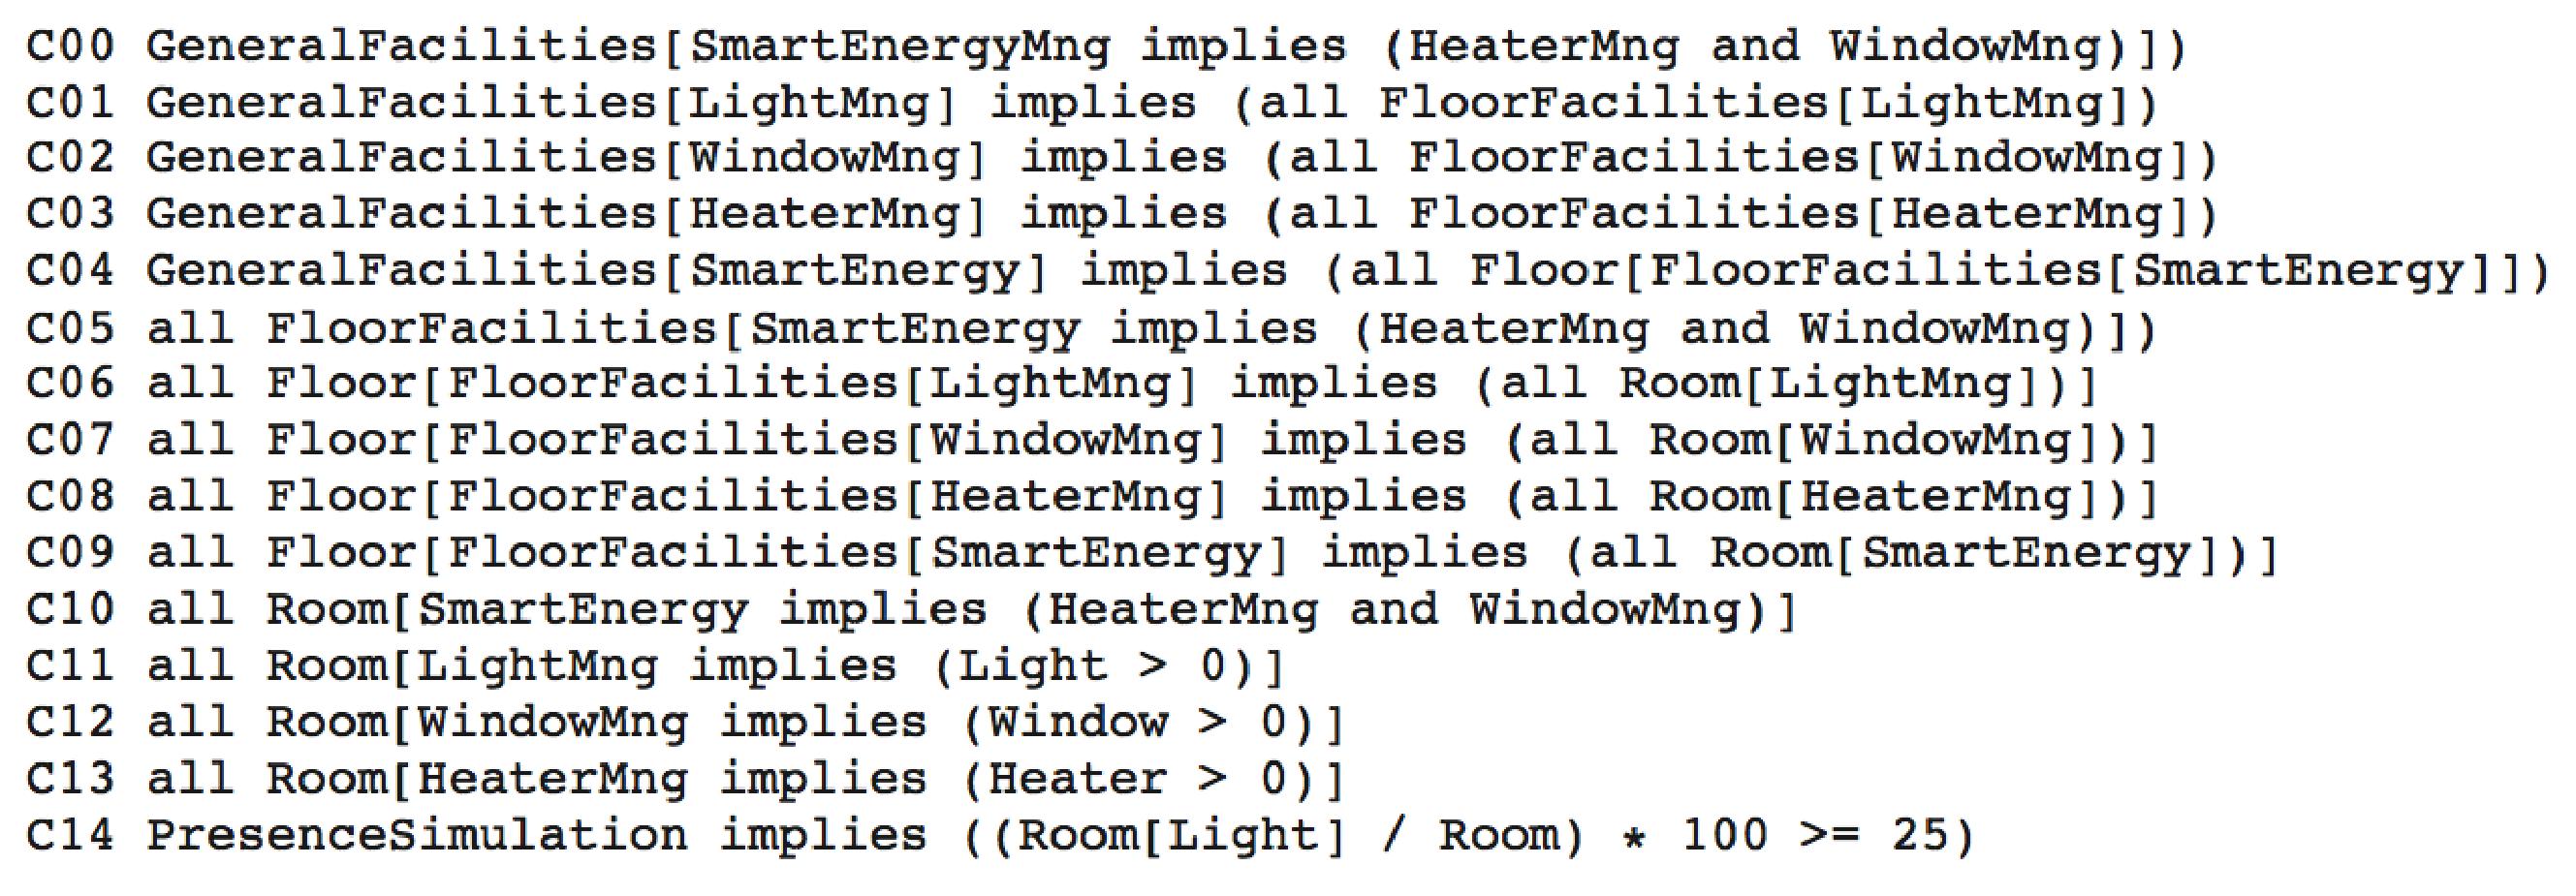
\includegraphics[scale=0.5]{gramatica/oppruebas.eps}
\caption{Bater�a de instrucciones para probar el funcionamiento de la gram�tica}
\label{figgrampruebas}
\end{figure}

Para hacer las pruebas correspondientes a la gram�tica fue de mucha utilidad la vista Outline de Eclipse, que permite obsevar el �rbol de parsing de todos los ficheros de c�digo que creemos en nuestro lenguaje. 

La bater�a de pruebas simplemente consisti� en comprobar una serie de instrucciones y observar dentro de la vista Outline si se parseaban de modo correcto. En este caso se utilizaron unas restricciones definidas en un documento previo de Hydra que conten�an todos los aspectos problem�ticos de la gram�tica, es decir, operaciones largas con prioridad y multitud de contextos. Estas instrucciones son las que se muestran en la figura \ref{figgrampruebas}. 

El resto de operaciones fueron puestas a prueba con restricciones m�s sencillitas y, como en el caso anterior, fueron exitosas. Tambi�n se usaron las instrucciones de las pruebas del cap�tulo anterior, que se pueden observar en la figura \ref{figmetains} para comprobar que el �rbol era el mismo que se cre� en ese momento.

\section{Sumario}
\label{sec:meta:sumario}
